\documentclass{standalone}
\usepackage{tikz}
\usetikzlibrary{arrows.meta}
\tikzset{label/.style = {inner sep=1pt, fill=white}}
%\tikzset{nd/.style={circle, inner sep=0pt}}
\tikzset{nd/.style={inner sep=1pt}}
\tikzset{>=Latex}
\tikzset{arc/.style = {->, semithick, >=Latex}}
\begin{document}
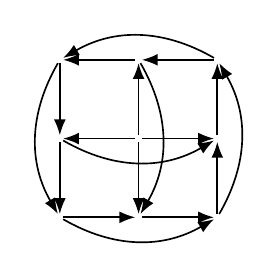
\begin{tikzpicture}

    \node[nd] (1) at (0,0) {};
    \node[nd] (2) at (1,0) {};
    \node[nd] (3) at (2,0) {};
    \node[nd] (4) at (0,1) {};
    \node[nd] (5) at (1,1) {};
    \node[nd] (6) at (2,1) {};
    \node[nd] (7) at (0,2) {};
    \node[nd] (8) at (1,2) {};
    \node[nd] (9) at (2,2) {};
    
    \draw[arc] (4) to (1);
    \draw[arc] (1) to[out = -30, in = 210] (3);
    \draw[arc] (3) to[in = -60, out = 60] (9);
    \draw[arc] (9) to (8);
    \draw[arc] (5) to (8);
    \draw[arc] (5) to (4);
    
    \draw[arc] (7) to (4);
    \draw[arc] (7) to[out = -120, in = 120] (1);
    \draw[arc] (8) to (7);
    \draw[arc] (9) to[out = 150, in = 30] (7);
    \draw[arc] (1) to (2);
    \draw[arc] (2) to (3);
    \draw[arc] (5) to (2);
    \draw[arc] (8) to[out = -60, in = 60] (2);
    \draw[arc] (3) to (6);
    \draw[arc] (6) to (9);
    \draw[arc] (5) to (6);
    \draw[arc] (4) to[in = 210, out = -30] (6);
 \end{tikzpicture}
\end{document}